%%%%%%%%%%%%%%%%%%%%%%%%%%%%%%%%%%%%%%%%%%%%%%%%%%%%%%%%%%%%%%%%%%%%%%%%%%%%%%%%%%
\begin{frame}[fragile]\frametitle{}
\begin{center}
{\Large Introduction to LangGraph}
\end{center}
\end{frame}

%%%%%%%%%%%%%%%%%%%%%%%%%%%%%%%%%%%%%%%%%%%%%%%%%%%%%%%%%%%%%%%%%%%%%%%%%%%%%%%%%%
\begin{frame}\frametitle{What is LangGraph?}

\begin{itemize}
\item Building state-ful multi agent applications using LLMs (Large Language Models)
\item So, components are not in `chain' as in LangChain (ie Sequential) but can a Graph.
\item Like Workflow modeling or orchestration
\end{itemize}

\begin{center}
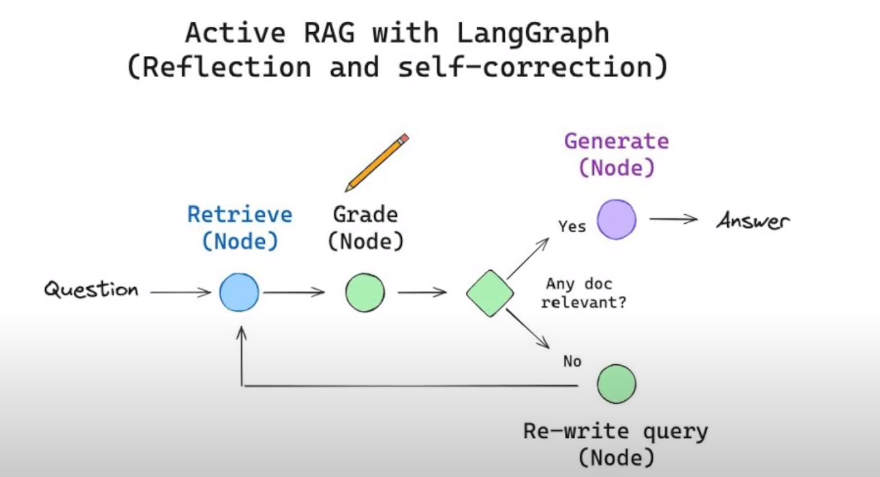
\includegraphics[width=0.8\linewidth,keepaspectratio]{langgraph1}
\end{center}	  


{\tiny (Ref: Introduction to LangGraph | Building an AI Generated Podcast - Prompt Circle AI)}
\end{frame}

%%%%%%%%%%%%%%%%%%%%%%%%%%%%%%%%%%%%%%%%%%%%%%%%%%%%%%%%%%%%%%%%%%%%%%%%%%%%%%%%%%
\begin{frame}\frametitle{Concepts}

\begin{itemize}
\item Model: Large Language Model that supports Function Calling
\item Tools: Actions taken by app, ie API calls, Db operations, etc
\item State: Represents info that is carried though out the workflow e.g Message State has list of messages produced from each Node.
\item Node: executable logic container, a Langchain runnable or a Tool invoker. Nodes are connected by edges.
\item Edge: control flow of info, conditional or normal
\item Workflow: The graph, having nodes and edges, can be invoked or streamed from.
\end{itemize}

\begin{center}
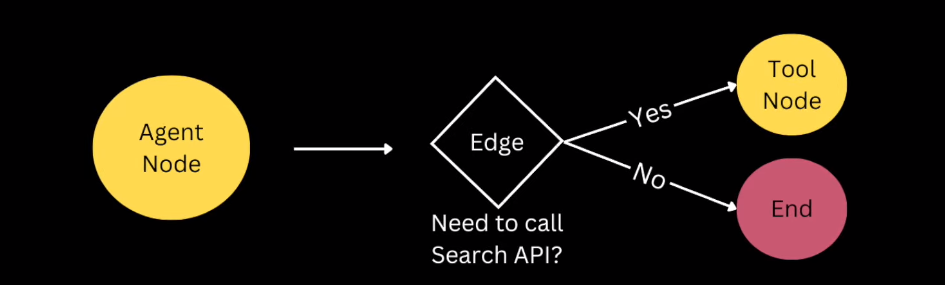
\includegraphics[width=0.8\linewidth,keepaspectratio]{langgraph2}
\end{center}	  

{\tiny (Ref: Introduction to LangGraph | Building an AI Generated Podcast - Prompt Circle AI)}
\end{frame}

%%%%%%%%%%%%%%%%%%%%%%%%%%%%%%%%%%%%%%%%%%%%%%%%%%%%%%%%%%%%%%%%%%%%%%%%%%%%%%%%%%
\begin{frame}[fragile]\frametitle{Why LangGraph?}

\begin{itemize}
\item Most of the Multi-agent frameworks are rigid, monolithic
\item LangGraph decouples the agents from their orchestration.
\item Here, agents can have different LLMs, can combine even non-LLM services together, can combine agents from other systems such as Autogen or Crew AI etc.
\end{itemize}


{\tiny (Ref: Langgraph: The Agent Orchestrator - Rajib Deb)}

\begin{lstlisting}
agent_1 = MyAgent("agent_1")
agent_2 = MyAgent("agent_2")
group_chat = [agent_1,agent_2]
group_chat.invoke("What is GST?")
\end{lstlisting}

\end{frame}
